\subsection{HA Barbarossa}


\begin{center}
    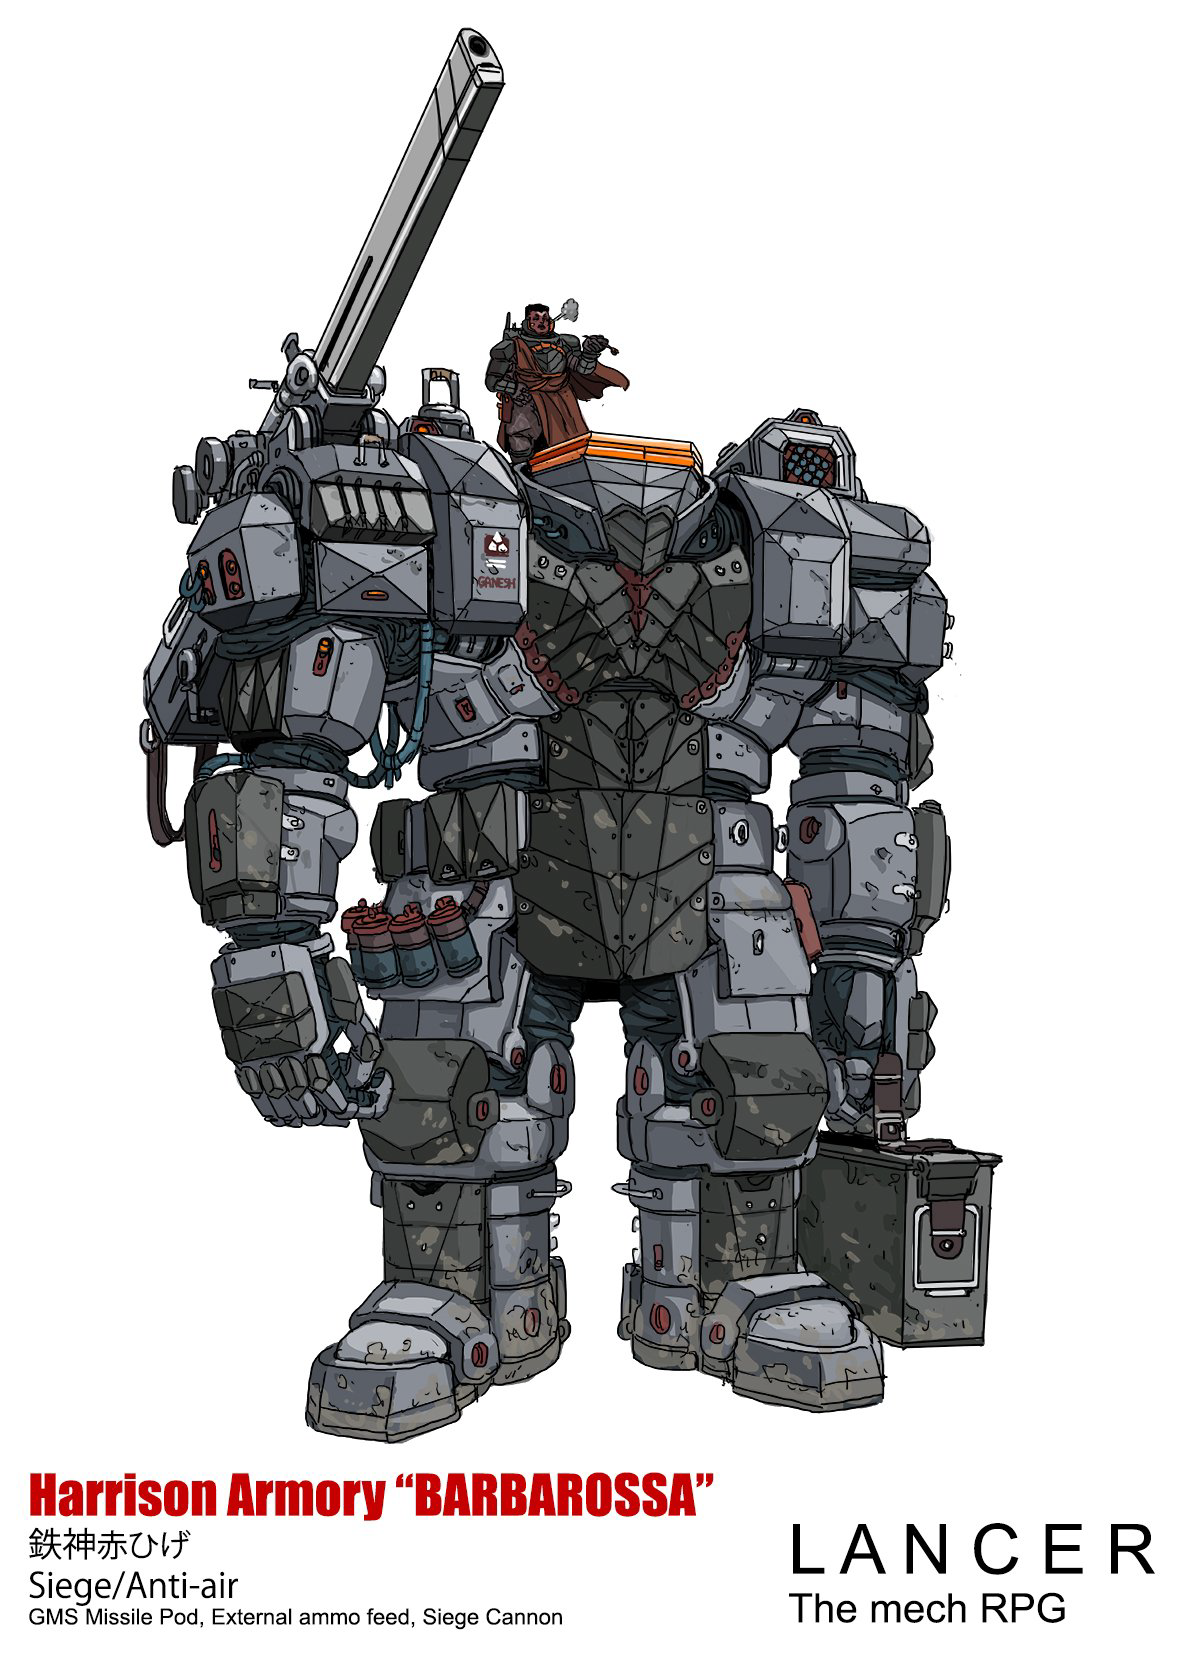
\includegraphics{Barbarossa}
\end{center}

                           HARRISON ARMORY BARBAROSSA

The BARBAROSSA chassis is a massive frame, built to carry the heaviest of weapons and equipment.

Standing nearly forty feet tall at its highest point, the BARBAROSSA is a slow, unsubtle beast of a mech,
inspiring terror in enemies and comfort in allies. The weapons it can mount are capable of going toe-to-toe
with corvette and cutter class ships; indeed, due to its size and slow maneuverability, the BARBAROSSA is




commonly employed in micro and zero gravity engagements where mass is less of a factor. The
BARBAROSSA is rated for all theaters, and excels in ranged combat situations.

                                                  License:

I. Siege Stabilizers, Roller Grenades

II. BARBAROSSA FRAME, Auto-Loader, Flak Cannon

III. External Ammo Feed, Siege Cannon


                                            BARBAROSSA

 HP: 10         Evasion: 6                           Speed: 2           Heat Cap: 7       Sensors: 10

 Armor:  2      E-Defense: 6                         Size: 3            Repair Cap: 4     Tech Attack:
                                                                                          +0

                                                  TRAITS:

 Heavy FRAME: The Barbarossa cannot be knocked back or prone by actors smaller than itself

 Siege Shield: The Barbarossa has resistance to Explosive Damage

 Slow: The Barbarossa gets +1 Difficulty on Agility checks

                                           SYSTEM POINTS: 5

                                                 MOUNTS:

 Main Mount                                          Apocalypse Rail

                                              CORE system




                                                Apocalypse Rail

 The HA Apocalypse Rail is a spinal mount augmentation that adapts the weapon mounted upon it to
 patch directly into its host mech’s coldcore. This allows for energy conservation/overcharge cycling:
 most effective with energy weapons, this system allows a pilot to dump excess offensive energy from
 sub-super weapons and systems into its central core, exciting the cold-burn system into an overcharge
 state, which is then used to overpower and override inherent limiters built into the factory spec weapon
 mounted in the Apocalypse Rail. This overcharge state allows for momentary overclocking of the AR-
 mounted weapon, sacrificing mobility and auxiliary abilities in favor of stationary defense and attack.

 Passive: Your mech has the apocalypse rail, a weapon mount that takes a superheavy or smaller sized
 weapon. You can still mount smaller weapons on the apocalypse rail. You don’t need an additional
 mount to add a superheavy weapon to this mount. This mount is not modifiable (such as from core
 bonuses).


 Active (requires 1 core power): Convert to Battery
 Quick Action

 Your mech converts to something more resembling a gun emplacement. While this mode is active, you
 have the following drawbacks:

      -   Your mech is immobilized

      -   You cannot directly attack any target within range 5 of your mech

      -   You can only make attacks with the weapon mounted in your Apocalypse Rail

 However, you gain the following benefits:

      -   You cannot be moved (such as with a grapple) by any target smaller than you

      -   You have resistance to heat

      -   The weapon mounted in your Apocalypse Rail can be fired twice with the Barrage action
          instead of just once. If it has the loading tag, it can still be fired twice (but must be reloaded
          normally after)

Siege Stabilizers

Some weapons require further stabilization for optimal use: with Armory-sanctioned Siege Stabilizers
installed, a chassis becomes a stable firing platform for any weapon.

1 SP
Quick Action

Extend or retract your stabilizers as a quick action. Your mech is immobilized while this system is
active, but you can increase the base range of your ranged weapon attacks by +5. You cannot
directly target any target within range 5 when this system is activated.


Roller Grenades

2 SP, Limited (2)
Quick Action, Grenade
Instead of throwing these grenades normally, draw a line 15 spaces long from your mech. These
grenades bounce over cover and objects up to size 1, and can pass through holes or areas as
small as size 1/2. They detonate when they move through or adjacent to any actor’s space (even
allied ones), dealing 2d6 explosive damage to that target only and knocking that actor back in




the direction of the line 3 spaces. The target can pass an agility check to avoid the knock back
and halve the damage.


Auto-Loader Drone

Auto-Loader Drones are half-size, many-legged arthropod-analogous drone systems that assist
sectionmate chassis in loading ordinance, maintaining powerline hookups, and cycling magazine-fed

weapons.

2 SP, Limited (1)
Drone
This drone can be deployed in an adjacent space. While deployed, once per round, any one
adjacent mech can reload a weapon with the Loading tag as a quick action. It lasts until the end
of the current scene, then deactivates.


Flak Cannon
A quad-barreled autocannon, flak cannons are loaded with proximity-explosive shells perfect for
blanketing fire. A perfect weapon for use against massed infantry or low-altitude flyers.

Main Cannon

Reliable 1

Range 20

1d3 Kinetic Damage

Any flying target hit by this weapon must pass an agility check or immediately fall.

External Ammo Feed


An EAF is a general term for any manner of additional ammunition not carried in a chassis‘s integrated
storage. Whether in magazines strapped to brachial, trunk, or ambulatory elements; battery packs attached

to hip clasps; or massive, dorsal-mount ammunition/ charge packs, an EAF ensures that you‘ll have more
than enough boom to get the job done.

3 SP, Unique

Once on your turn, you can take 1d3+1 heat to reload any weapon with the Loading tag as a
quick action


Siege Cannon

Siege Cannons are the Armory‘s core-squadron level artillery, a howitzer-style 10“ gun fed by a self-
contained loading system. Commonly mounted on rear-line mechs deployed in an artillery/ squad support
role, the Siege Cannon is capable of direct fire should the necessities of dynamic combat call for it. Siege

cannons can fire HE and canister FRAMEs, depending on the target.

Superheavy Cannon

4 heat (self), Arcing, Ordnance, Loading

Range 30, Blast 2

3d6 explosive damage

